\section{Lab Task - First OpenPLC Program}
In \textbf{Understanding Check \#2} you were asked to calculate the output for Figure~\ref{fig:understanindCheck2}. Using the OpenPLC Editor, your task is to verify your answers from \textbf{Understanding Check \#2}, by creating and executing a ladder diagram. Figure~\ref{fig:understanindCheck2} is repeated here for your reference.

\begin{figure}[!thb]
\begin{center}
\tcbox[colframe=black,colback=white!30]{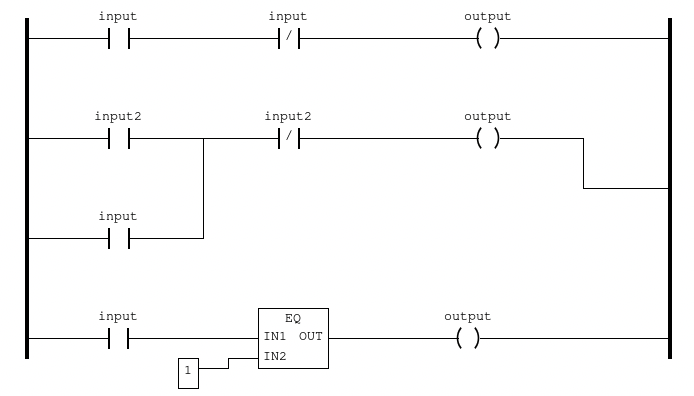
\includegraphics[width=.76\textwidth]{./images/LadderDiagram06.png}}
\end{center}
% \caption{Ladder Diagram for Understanding Check \#2}
\repeatcaption{fig:understanindCheck2}{}
\end{figure}

\subsection{Specifications}
You will submit a single PDF that will contain your answers from \textbf{Understanding Check \#2} and screen captures from the OpenPLC Editor. Place your name and the lab number at the top of the page in the upper left hand section of the header. Your sections will be labeled using the title from each bullet below.

\begin{itemize}[listparindent=1.5em]
    \item \textbf{Section 1 - Understanding Check \#2 Answers}
        
        Copy your truth table and answers to the questions from Understanding Check \#2.
    
    \item \textbf{Section 2 - Ladder Diagram}
        
        Open the OpenPLC Editor and create a project named Lab0. Only create the ladder diagram shown in  Figure~\ref{fig:understanindCheck2}. Take a screen capture of the ladder diagram and paste the image under this section.
    
    \item \textbf{Section 3 - Variable Declarations}
        
        In the OpenPLC editor add the variables as specified in the ladder diagram.  You must determine the appropriate types for input, input2, and output. Once you have declared all your variables take a screen capture of the variable section and paste the image under this section. Write at least two sentences justifying why you chose the variable type for input, input2, and output.
    
     \item \textbf{Section 4 - Executing and Debugging your Ladder Diagram}
        
        In the upper left project window click on the program named lab0. In the configuration window on the lower left your variables will appear.  Next click on the glasses next to each variable. clicking on the glasses next to the variable, will add your variables to the debugger window. 
     
        Next run your program by clicking on the Running Figure to the left of the variable bar. Watch your variables in the debugging window and not the initial state of the variables and output. Based on your answers to Understanding Check \#2 toggle the variables and verify your answers.
        
        Take at least two screen captures of the debugger window illustrating the toggling of your variables, and changing of your output value.
     
     \item \textbf{Section 5 - Lab Summary}
     
        Write a summary paragraph explaining your Understanding Check \#2 answers versus the actual results from your PLC program.  This discussion should include any challenges you encountered in creating the ladder diagram, variables, and running your code. 
     
\end{itemize}

\subsection{Submission}
Submit your single PDF before the required due date and time. Name your PDF your last name first letter of your first name Lab0.pdf. (Example: steinersLab0.pdf)
